\chapter{Growth technique}
\label{sec:growth}

% Description of various techniques. 
% FSGP
	% Uses sublimation
	% Different polytypes at different pressures
	% Setup
		% Describe the figure
	% Substrate
		% Off axis (compare on-axis) 
		% Cleaned
% Parameter space
	% Describe from book
	% Review of what has been done in group
% Growth of doped material. 

SiC can be fabricated by several different techniques, and the different techniques are advantageous for different polytypes and applications. Some of the most common methods are \emph{sublimation epitaxy}, \emph{liquid phase epitaxy (LPE)}, \emph{chemical vapour deposition (CVD)} and \emph{physical vapour deposition (PVD)} \cite{Ivanov1999}. 

The goal when growing freestanding material is to have high quality material of large volume. Up to this point in time, researchers have had more success fabricating high quality 4H and 6H material compared to 3C \cite{J.B.CASADYandR.W.JOHNSON1996}. The hexagonal polytypes are commonly fabricated using PVD. This method has not been widely adapted to 3C growth however, which is often attributed to the fact that this method uses homoepitaxy, and there are no 3C seeds widely available. Historically in the growth of 3C using CVD, there has been a trade-off between crystal quality and growth rate. Nishino et al. reported in 1983 a growth rate of approximately 2.5 microns per hour with the CVD technique for 3C growth \cite{Nishino1983}. This rate is much too low to create free standing material. The growth rate for CVD growth has been improved since this time, and in 2002 Nagasawa et al. reported a rate of 40 $\mu$m/h \cite{Nagasawa2002}, which makes it possible to fabricate free standing 3C. 

Another growth method is sublimation epitaxy, which was demonstrated by Lely in 1955 \cite{Lely1955}. In this method material is transferred between a source material and a substrate using the fact that SiC sublimes. Recently there have been reports of high quality cubic SiC fabricated by a type of sublimation epitaxy called \emph{fast sublimation epitaxy (FSGP)}. Growth rates as high as 500 $\mu$m/h have been reported using this method, while still having good quality material \cite{Jokubavicius2014}. This high growth rate is obviously ideal for growth of free standing (and even bulk) material. This chapter describes in detail the sublimation method in general and FSGP in particular. FSGP is the method used to obtain the results in this thesis. 
 
 \section{About sublimation and nucleation}
 % What is sublimation, how does it work?
 % What governs the process?
 Sublimation is the phase transition where a material transitions between solid and gas, without the intermediate liquid phase. At normal conditions SiC does not melt, but rather it sublimes. For SiC to melt a pressure of 100,000 atm and a temperature of at least 3200 $^\circ$C is required. At atmospheric pressure SiC can only sublime \cite{Scheel2003}. Sublimation of a SiC source material will give a vapour consisting of different molecules consisting of silicon and carbon, for example $\mathrm{Si, Si_2C, SiC_2}$ etc. The composition and vapour pressure of the gas can be controlled using parameters such as temperature and pressure of the ambient. 
 
If a substrate is placed in the silicon-carbon vapour some of the material will be adsorbed on the surface of the substrate, in the form of \emph{adatoms}. When many such atoms are adsorbed at the surface they bind together, forming a \emph{nucleus} of crystal growth. In a sublimation growth setup, a source of SiC is heated, initiating the sublimation. The vapour then travels to an appropriate substrate, by the means of a heat gradient. Material is adsorbed on the substrate which forms the grown crystal. Figure \ref{fig:sublimation} shows a schematic of this process. 

\begin{figure}[h]
\begin{center}
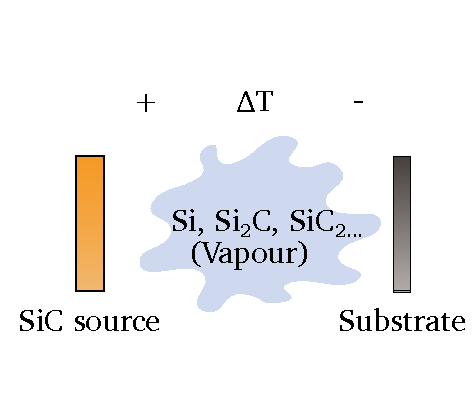
\includegraphics[scale=1]{sublimation.pdf}
\caption{A vapour containing silicon and carbon molecules is created by sublimation of a SiC source. The vapour is adsorbed at the substrate. 
\label{fig:sublimation}}
\end{center}
\end{figure}
 
 As the material is adsorbed at the substrate the growth begins. The crystal growth is governed by the free energy of the whole system. A decrease in free energy works to promote the growth. In crystal growth, a decrease in free energy is also a decrease in chemical potential $\mu$, meaning that crystal growth is driven by a decrease in chemical potential. The system is made up by the vapour and the crystal phases. Hence a change in chemical potential is given by 
 \[\Delta \mu = \mu_v -\mu_c,\]
where $\mu_v$ is the chemical potential for the vapour and $\mu_c$ is for the crystal. For growth from vapour phase, the chemical potential difference between vapour and crystal is dependent on the \emph{vapour pressure} and the \emph{saturated vapour pressure} through the formula
 \[\Delta \mu = k_BT\log(p/p_e),\]
where p is the vapour pressure and p$_e$ is the saturated counterpart. Defining the \emph{supersaturation}, $\sigma$, as
\[\sigma = \frac{p-p_e}{p_e}\]
thus
 \[\Delta \mu = k_BT\log(\sigma+1).\]
Taking the first order Taylor expansion around $\sigma = 1$ this becomes
\[\Delta \mu \approx k_BT\sigma.\]
 It is concluded that the change in chemical potential is directly proportional to the supersaturation of the system. A decrease in supersaturation will hence promote growth and, as shown below, increase growth rate. 
 
 Growth of the crystal can occur in several ways. One such way is called \emph{lateral enlargement} or simply \emph{lateral growth}. This growth mode is present on smooth surfaces. For growth to occur there must exist a place where the adatoms can bind to the surface. One such place is at a step on the surface. Steps on the surface will contain \emph{kinks}, which can be described as corners in the step. An adsorbed adatom diffuses on the surface until it encounters such a step kink, where it attaches. As atoms are bound to the step, it moves forward with a certain velocity. This velocity can be shown \cite{Scheel2003} to be
\[v_{\infty} = \frac{2\lambda_s}{n_0}\frac{p_e}{\sqrt{2\pi mk_BT}}\sigma.\]

Here $\lambda_s$ is the diffusion length of an adatom before it gets desorbed from the surface. Moreover $n_0$ is the density of lattice points on the surface and m is the atom mass. It is important to note that the step velocity, and hence the growth rate, is linearly proportional to the supersaturation. 
 
 
% \section{Growth using FSGP}

 


 
 
 
 
 
 
 
 
 
 
 
 
 
 
 
 
 
 
 
 
 
 
 
 
 
 
 
 
 
 
 
 
 
 
 
 
 
 
 
 
 
 
 